
We performed the LVG analysis with the radiative transfer code RADEX developed by \citet{2007A&A...468..627V}. The simulation constructs a large grid of non-LTE models with three parameters: gas density ($n_{\mathrm{H}_2}$), kinetic temperature ($T_{\mathrm{kin}}$), and the ratio between column density and line width ($N_{\mathrm{CO}}$/$\Delta V$). Considering the velocity resolution of our observations, we fix $\Delta V$ to 2 km s$^{-1}$. Each model gives the prediction of the brightness temperature ($T_\mathrm{b}$) of different CO transitions. Then we measured the main beam temperature ($T_{\mathrm{mb}}$) of four CO lines extracted at the peak position of the blue lobe and the red lobe (marked as two crosses in Figure \ref{fig1}). So we could compare the simulated $T_\mathrm{b}$ with our measured $T_{\mathrm{mb}}$, as $T_{\mathrm{mb}}$ is related to $T_\mathrm{b}$ by the relation:
\begin{equation}
T_{\mathrm{mb}} = \frac{\Omega_{\mathrm{s}}^2}{\Omega_{\mathrm{s}}^2+\Omega_{\mathrm{mb}}^2}\times T_\mathrm{b} = f_{\mathrm{b}} \times T_\mathrm{b},
\end{equation}
where $\Omega_{\mathrm{s}}$ and $\Omega_{\mathrm{mb}}$ are the source size and the beam size in arcsec, and $f_{\mathrm{b}}$ is the beam filling factor. Given the complex structures of G240 outflow at higher resolution \citep{2009ApJ...696...66Q}, we cannot get a good estimate of the source size. Then the beam filling factors are assumed to be the same for all transitions, and fixed to 1, during our analysis. Thus, the derived physical parameters of the gas are beam-averaged values. We would further discuss how the beam dilution affect our results in the following part of this section.

We report the results from a $\chi^2_{\mathrm{red}}$ fitting. $\chi^2_{\mathrm{red}}$ is the reduced $\chi^2$: 
\begin{equation}
\chi^2_{\mathrm{red}} = \frac{1}{N - n} \sum_{i=1}^{4}(I_o - I_m)^2/\sigma^2,
\end{equation}
where $N$ is the number of observed intensities, $n$ the number of fitted parameters, $I_\mathrm{o}$ the observed intensity, $I_\mathrm{m}$ the modelled intensity, and $\sigma$ is the uncertainty of the observed intensity. With four line observations and three simulation parameters, our fitting has one degree of freedom. Considering the calibration error and pointing accuracy of our CO observations, we set the intensity uncertainty of CO (2-1), CO (3-2), CO (6-5), CO (7-6) to 0.15, 0.2, 0.25, 0.3 respectively. The best fit is then obtained by minimizing the $\chi^2_{\mathrm{red}}$ between the observed and modelled data using the Levenberg-Marquardt method \citep{1992nrfa.book.....P}. However, at velocities where no CO (7-6) emission is detected, the best fit is obtained by minimizing $\chi^2$ instead of $\chi^2_{\mathrm{red}}$. Then we found the best fitting result at most velocities has a $\chi^2_{\mathrm{red}}$ less than 1, indicating that we might be a bit conservative at the intensity uncertainty or the real value of degrees of freedom is smaller than one \citep{2010arXiv1012.3754A}. So we divided $(N - n)\sigma^2$ by an appropriate factor to make $\chi^2_{\mathrm{red}}$ approach 1 at most velocities. At some velocities, the $\chi_{\mathrm{red}}^2$ remains much less than 1 even after our adjustment of intensity uncertainty, which can account for the anomaly high upper limits of gas temperature at these velocities in Figure \ref{fig4a}. 

\begin{figure}[tbp]
\centering
\subfigure[]{
\begin{minipage}[b]{0.5\textwidth}
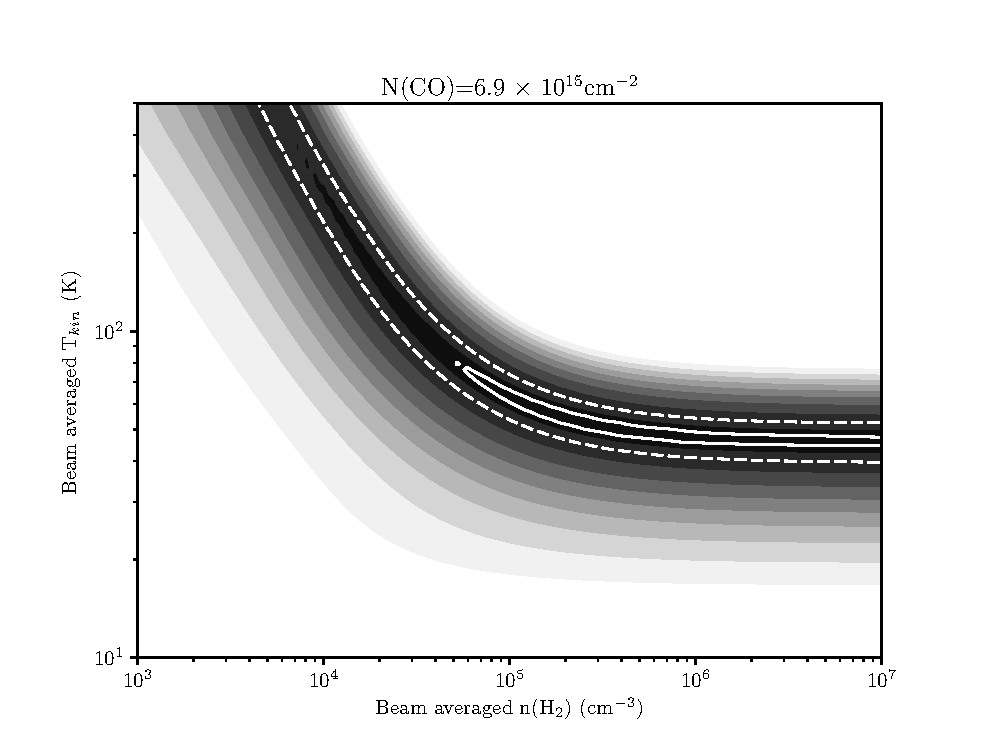
\includegraphics[width=1\textwidth]{./fig/chiimage_nco_paper.eps}
\label{fig3a}
\end{minipage}
}
\subfigure[]{
\begin{minipage}[b]{0.5\textwidth}
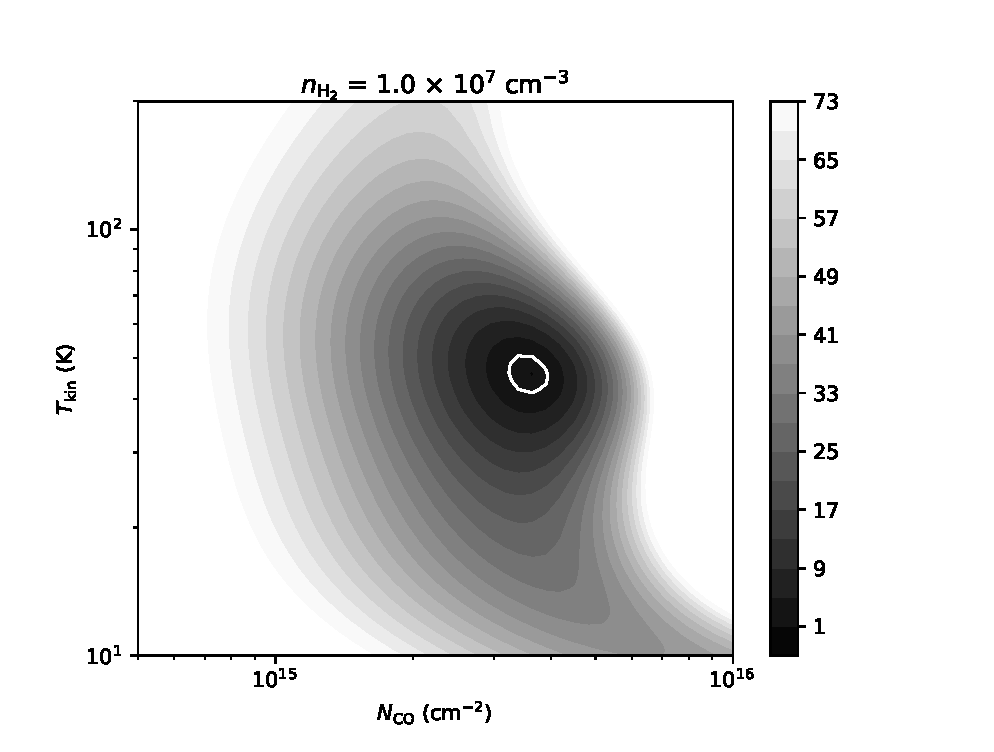
\includegraphics[width=1\textwidth]{./fig/chiimage_nh2_paper.eps}
\label{fig3b}
\end{minipage}
}
\subfigure[]{
\begin{minipage}[b]{0.5\textwidth}
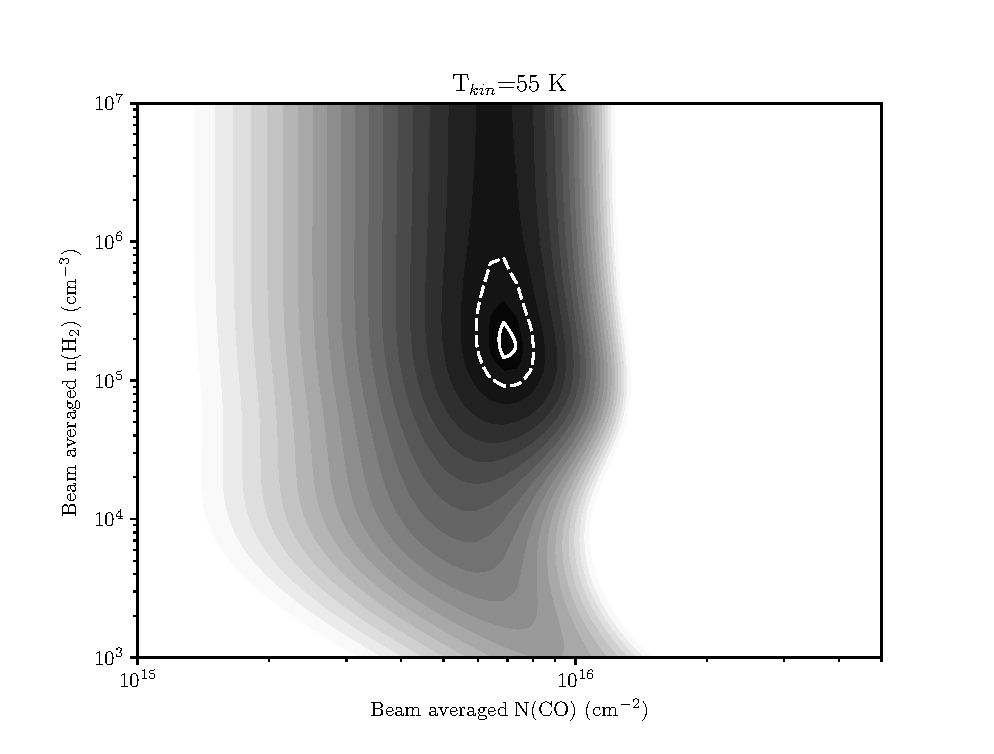
\includegraphics[width=1\textwidth]{./fig/chiimage_tkin_paper.eps}
\label{fig3c}
\end{minipage}
}
\caption{The $\chi_{\mathrm{red}}^2$ distribution for G240 outflow at 58 km s$^{-1}$ in the (a) [$T$, $n$], (b) [$T$, $N$], (c) [$n$, $N$] planes, with all other parameters fixed to the parameters of the best fitting results at this velocity. Solid contours and dashed contours show the 1$\sigma$ and 3$\sigma$ confidence levels respectively. \label{fig3}}
\end{figure}

In Figure \ref{fig3}, we show cuts in the $\chi_{\mathrm{red}}^2$ along the [$T$, $n$], [$T$, $N$], [$n$, $N$] planes for 58 km s$^{-1}$ as an example of the $\chi_{\mathrm{red}}^2$ distribution, with all the other parameters fixed to  the parameters of the best fitting result at this velocity. The $\chi_{\mathrm{red}}^2$ distribution in [$T$, $n$], [$T$, $N$] planes is well behaved, with only one minimum, as shown in Figure \ref{fig3b} and Figure \ref{fig3c}. However, Figure \ref{fig3a} shows that the gas might be thermalized and no upper limits to the density could be derived. The $\chi_{\mathrm{red}}^2$ distribution behaves similarly at other velocities. 

\begin{figure}[htbp]
\centering
\subfigure[]{
\begin{minipage}[b]{0.5\textwidth}
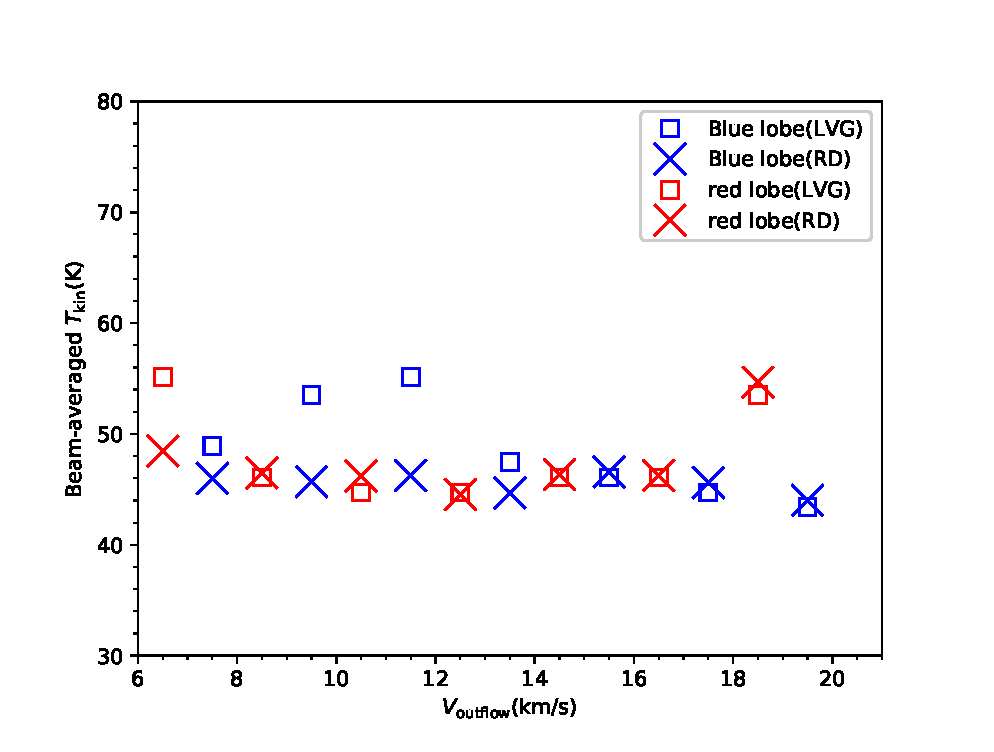
\includegraphics[width=1\textwidth]{./fig/tv_paper.eps}
\label{fig4a}
\end{minipage}
}
\subfigure[]{
\begin{minipage}[b]{0.5\textwidth}
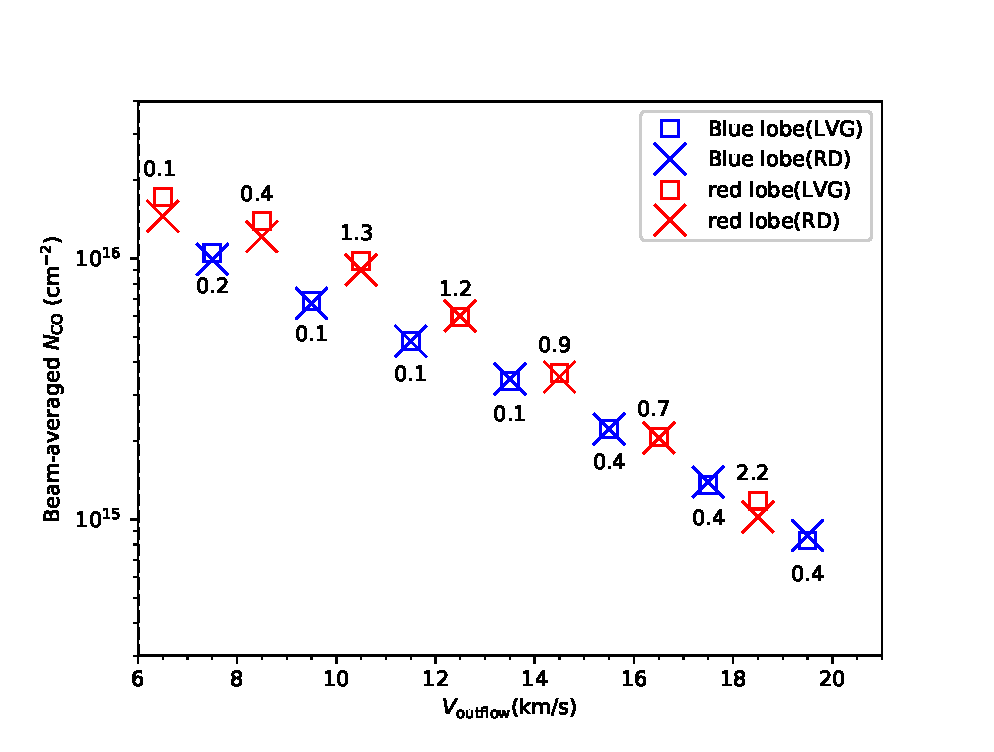
\includegraphics[width=1\textwidth]{./fig/Nv_paper.eps}
\label{fig4b}
\end{minipage}
}
\caption{$T$-$V$ and $N$-$V$ diagrams of the G240 outflow, estimated from LVG analysis (black circles for blue lobe and black squares for red lobe) and population diagram analysis (cyan x marker for blue lobe and red x marker for red lobe). The 1$\sigma$ temperature uncertainty estimated from the LVG analysis is represented in the $T$-$V$ diagram (error bars). \label{fig4}}
\end{figure}

We also performed a population diagram analysis with the assumptions of local thermal equilibrium (LTE) and low opacity, and derived the kinetic temperature of the outflow gas and the CO column density as a function of velocity \citep{1999ApJ...517..209G}. Figure \ref{fig4} shows the outflowing gas temperature and CO column density, estimated from the LVG analysiss and population diagram analysis, versus outflowing gas velocity. The $N$-$V$ diagram shows a clear decreasing trend of CO column density with outflow velocity, while the $T$-$V$ diagram shows that the gas temperature has no obvious dependence on gas velocity. Uncertainty of each parameter in the LVG analysis is derived from the 1$\sigma$ confidence region in the $N$-$T$-$n$ 3-dimensional space. The 1$\sigma$ temperature uncertainty of the LVG analysis is shown in Figure \ref{fig4a}, at velocities where all of the four lines are detected. The uncertainty of the CO column density is too small to be plotted, so we don't show it in Figure \ref{fig4b}. The lower limits of gas density ($n_{\mathrm{lower}}$) are around 10$^5$ cm$^{-3}$ at most velocities. At velocities where $\chi_{\mathrm{red}}^2 \ll 1$, $n_{\mathrm{lower}}$ could be as low as $3 \times 10^4$ cm$^{-3}$.

To explore how the effect of beam dilution influence our results, we varied the beam filling factors from 0.2 to 1. Then we performed the LVG analysis again, and compared the simulated $T_\mathrm{b}$ with the corrected antenna temperatures ($T_{\mathrm{mb}}$ divided by a beam filling factor). We find that modelling with different beam filling factors mainly affect the $N$-$V$ diagram, with minor change in the $T$-$V$ diagram and density limits. This could be resulted from the degeneracies of the beam filling factor with CO column density in the optically thin case. 